\documentclass[11pt]{article}
\usepackage[margin=1in]{geometry}
\usepackage{times}
\usepackage{tikz}
\usepackage{graphicx}
\usepackage{inconsolata}
\usepackage{xcolor}
\usepackage{float}
\usetikzlibrary{shapes.geometric, shapes.symbols, arrows.meta, positioning, calc, backgrounds}
\usepackage{wrapfig}
\usepackage{tcolorbox}
\tcbuselibrary{skins}

\definecolor{tealfill}    {HTML}{E1F5EE}
\definecolor{tealstroke}  {HTML}{0F6E56}
\definecolor{tealtext}    {HTML}{085041}
\definecolor{purplefill}  {HTML}{EEEDFE}
\definecolor{purplestroke}{HTML}{534AB7}
\definecolor{purpletext}  {HTML}{3C3489}
\definecolor{amberfill}   {HTML}{FAEEDA}
\definecolor{amberstroke} {HTML}{854F0B}
\definecolor{ambertext}   {HTML}{633806}
\definecolor{bluefill}    {HTML}{E6F1FB}
\definecolor{bluestroke}  {HTML}{185FA5}
\definecolor{bluetext}    {HTML}{0C447C}
\definecolor{coralfill}   {HTML}{FAECE7}
\definecolor{coralstroke} {HTML}{993C1D}
\definecolor{coraltext}   {HTML}{712B13}
\definecolor{greenfill}   {HTML}{EAF3DE}
\definecolor{greenstroke} {HTML}{3B6D11}
\definecolor{greentext}   {HTML}{27500A}
\definecolor{grayfill}    {HTML}{F1EFE8}
\definecolor{graystroke}  {HTML}{5F5E5A}
\definecolor{graytext}    {HTML}{2C2C2A}

\tikzset{
  procnode/.style={rectangle, rounded corners=6pt, minimum width=3.6cm,
    minimum height=1.0cm, align=center, text width=3.4cm,
    draw, line width=0.5pt, font=\small},
  dbnode/.style={cylinder, shape border rotate=90, minimum width=2.8cm,
    minimum height=1.1cm, align=center, text width=2.4cm,
    draw, line width=0.5pt, font=\small, aspect=0.25},
  teal/.style  ={fill=tealfill,   draw=tealstroke,   text=tealtext},
  purple/.style={fill=purplefill, draw=purplestroke, text=purpletext},
  amber/.style ={fill=amberfill,  draw=amberstroke,  text=ambertext},
  blue/.style  ={fill=bluefill,   draw=bluestroke,   text=bluetext},
  coral/.style ={fill=coralfill,  draw=coralstroke,  text=coraltext},
  green/.style ={fill=greenfill,  draw=greenstroke,  text=greentext},
  gray/.style  ={fill=grayfill,   draw=graystroke,   text=graytext},
  solidarr/.style={-{Latex[length=5pt,width=4pt]}, line width=0.8pt, color=graystroke},
  crossarr/.style={-{Latex[length=5pt,width=4pt]}, line width=1.0pt, color=tealstroke}
}
\newcommand{\sub}[1]{\\[2pt]{\footnotesize\color{graystroke}#1}}

\usepackage{url}
\usepackage[numbers]{natbib}
\usepackage{amsmath}
\usepackage{amssymb}
\usepackage{booktabs}
\usepackage{multirow}
\usepackage{subcaption}
\usepackage[toc,page]{appendix}
\usetikzlibrary{positioning, arrows.meta, calc, shapes, fit, matrix}

\title{\textbf{Trading Engagement for Sustainability:\\
Carbon-Aware Re-ranking for E-commerce Recommendations}\\[0.5em]
\large Midterm Project Report}

\author{}
\date{}

\begin{document}
\maketitle

%-----------------------------------------------------------------------
\section{Research Plan and Questions}
%-----------------------------------------------------------------------

E-commerce has become one of the dominant channels through which consumers
acquire goods, and its environmental consequences have attracted sustained
attention across dimensions including shipping logistics, packaging waste,
and return-driven reverse supply chains~\cite{olah2023sustainable}. UN
Trade and Development estimates global e-commerce sales reached USD~27
trillion in 2022~\cite{unctad2024ecommerce}, and the carbon consequences
of that volume are increasingly documented as a meaningful contributor to
greenhouse gas emissions~\cite{buldeorai2023ecommerce}.

Recommender systems sit at the centre of this problem. In large online
marketplaces, they determine which products become visible to users and
can therefore indirectly shape patterns of consumption~\cite{chaney2018confounding}.
By shaping the consideration set, algorithms can potentially shift demand
toward lower-impact alternatives without restricting user
choice~\cite{halimeh2026nudging}. This is the core motivation for
\emph{sustainability-aware recommender systems}, a growing research area
that incorporates environmental signals such as carbon footprint into
recommendation decisions~\cite{spillo2023greenerrec, spillo2023sustainabilityaware,
ecoa2026, vicenti2026pcfllm}.

One important sustainability signal is the Product Carbon Footprint (PCF),
typically measured in kilograms of CO$_2$ equivalent and estimated using
life-cycle assessment (LCA) methodologies~\cite{meinrenken2022carboncatalogue}.
Obtaining PCF values at scale is genuinely difficult: LCA studies require
extensive supply-chain data and are rarely available for the long tail of
products in large e-commerce catalogs~\cite{spillo2023greenerrec, ecoa2026}.
This project addresses this challenge directly by combining retrieval-based
PCF estimation with carbon-aware post-hoc re-ranking.

Our research questions are:

\begin{itemize}
  \item \textbf{RQ1:} How does carbon-aware re-ranking affect
    recommendation quality across different candidate generation models?
  \item \textbf{RQ2:} How much reduction in average recommended-item
    carbon footprint can be achieved while maintaining acceptable
    engagement performance?
  \item \textbf{RQ3:} Do different recommendation algorithms exhibit
    different engagement--sustainability trade-offs?
\end{itemize}

We evaluate these questions using the Amazon Reviews 2023, introduced in Hou et al~\cite{amazon2023}, across three product categories: Electronics,
Home and Kitchen, and Sports and Outdoors. Electronics results are
reported here; the remaining categories are in progress.

%-----------------------------------------------------------------------
\section{Methodology}
%-----------------------------------------------------------------------

Our framework follows a modular pipeline consisting of two sequential
components: a PCF estimation module and a carbon-aware recommendation
pipeline.

\begin{figure}[H]
  \centering
  \scalebox{0.78}{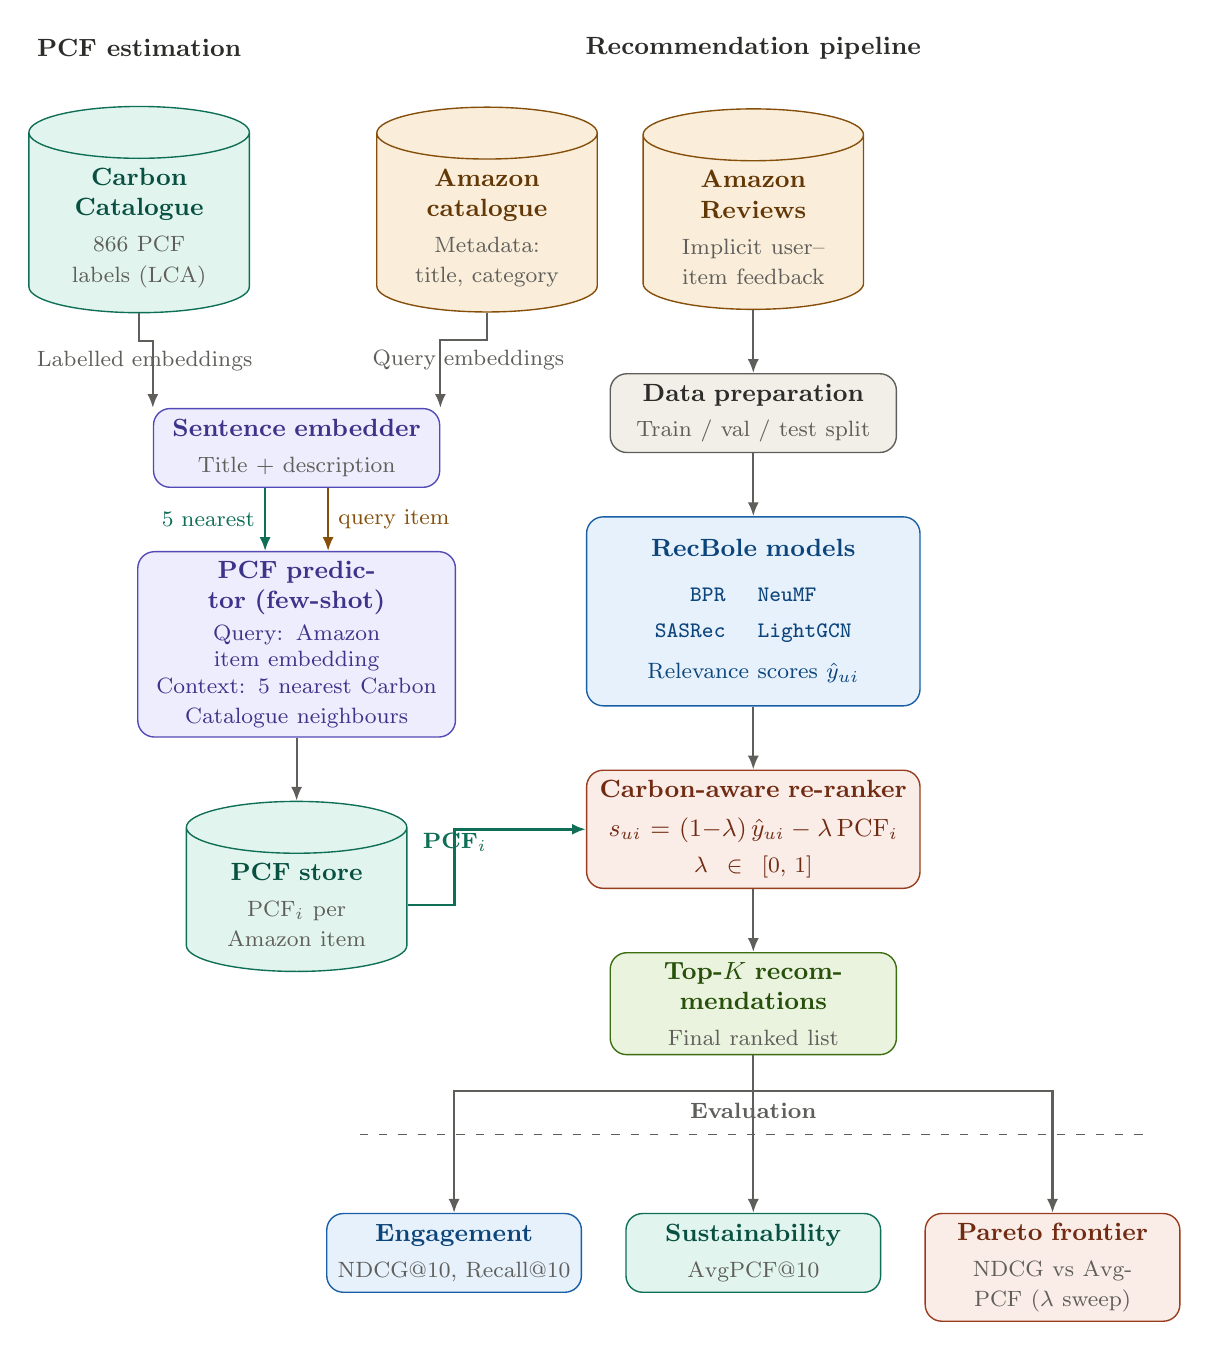
\begin{tikzpicture}[node distance=0.85cm]

  \node[font=\small\bfseries, text=graytext] (hdr-l) at (0, 0)
    {PCF estimation};
  \node[font=\small\bfseries, text=graytext] (hdr-r) at (7.8, 0)
    {Recommendation pipeline};

  %% LEFT COLUMN
  \node[dbnode, teal, below=0.5cm of hdr-l] (catalogue)
    {\textbf{Carbon Catalogue}\sub{866 PCF labels (LCA)}};

  \node[dbnode, amber, right=1.6cm of catalogue] (amazoncatalogue)
    {\textbf{Amazon catalogue}\sub{Metadata: title, category}};

  \node[procnode, purple, below=1.2cm of catalogue, xshift=2.0cm] (embedder)
    {\textbf{Sentence embedder}\sub{Title + description}};

  \node[procnode, purple,
        minimum height=1.3cm, text width=3.8cm, minimum width=4.0cm,
        below=0.8cm of embedder] (predictor)
    {\textbf{PCF predictor (few-shot)}\\[2pt]
     {\footnotesize\color{purpletext}
      Query: Amazon item embedding\\
      Context: 5 nearest Carbon\\
      Catalogue neighbours}};

  \node[dbnode, teal, below=0.8cm of predictor] (pcfstore)
    {\textbf{PCF store}\sub{PCF$_i$ per Amazon item}};

  \draw[solidarr]
    (catalogue.south) -- ++(0, -0.35)
    -| node[pos=0.2, below, font=\footnotesize, text=graystroke]
       {Labelled embeddings}
    (embedder.north west);

  \draw[solidarr]
    (amazoncatalogue.south) -- ++(0, -0.35)
    -| node[pos=0.2, below, font=\footnotesize, text=graystroke]
       {Query embeddings}
    (embedder.north east);

  \draw[solidarr, color=tealstroke]
    ([xshift=-0.4cm] embedder.south)
    -- node[left, font=\footnotesize, text=tealstroke] {5 nearest}
    ([xshift=-0.4cm] predictor.north);

  \draw[solidarr, color=amberstroke]
    ([xshift=0.4cm] embedder.south)
    -- node[right, font=\footnotesize, text=amberstroke] {query item}
    ([xshift=0.4cm] predictor.north);

  \draw[solidarr] (predictor) -- (pcfstore);

  %% RIGHT COLUMN
  \node[dbnode, amber, below=0.5cm of hdr-r] (reviews)
    {\textbf{Amazon Reviews}\sub{Implicit user--item feedback}};

  \node[procnode, gray, below=0.8cm of reviews] (dataprep)
    {\textbf{Data preparation}\sub{Train / val / test split}};

  \node[procnode, blue,
        minimum height=2.4cm, text width=4.0cm, minimum width=4.2cm,
        below=0.8cm of dataprep] (recbole)
    {\textbf{RecBole models}\\[5pt]
     {\footnotesize\ttfamily BPR \quad NeuMF}\\[2pt]
     {\footnotesize\ttfamily SASRec \quad LightGCN}\\[4pt]
     {\footnotesize\color{bluetext} Relevance scores $\hat{y}_{ui}$}};

  \node[procnode, coral,
        minimum height=1.5cm, text width=4.0cm, minimum width=4.2cm,
        below=0.8cm of recbole] (reranker)
    {\textbf{Carbon-aware re-ranker}\\[3pt]
     {\small $s_{ui} = (1{-}\lambda)\,\hat{y}_{ui} - \lambda\,\mathrm{PCF}_i$}\\[2pt]
     {\footnotesize\color{coraltext} $\lambda \in [0,\,1]$}};

  \node[procnode, green, below=0.8cm of reranker] (topk)
    {\textbf{Top-$K$ recommendations}\sub{Final ranked list}};

  \draw[solidarr] (reviews)  -- (dataprep);
  \draw[solidarr] (dataprep) -- (recbole);
  \draw[solidarr] (recbole)  -- (reranker);
  \draw[solidarr] (reranker) -- (topk);

  %% CROSS-COLUMN: PCF store to re-ranker
  \draw[crossarr]
    (pcfstore.east) -- ++(0.6, 0)
    |- node[pos=0.28, above, font=\footnotesize\bfseries, text=tealstroke]
       {PCF$_i$}
    (reranker.west);

  %% EVALUATION TIER
  \coordinate (divmid) at ($(topk.south) + (0, -1.0)$);
  \draw[graystroke, dashed, line width=0.4pt, dash pattern=on 3pt off 4pt]
    ($(divmid) + (-5.0, 0)$) -- ($(divmid) + (5.0, 0)$);
  \node[font=\footnotesize\bfseries, text=graystroke, anchor=south]
    at ($(divmid) + (0, 0.08)$) {Evaluation};

  \node[procnode, blue,
        minimum width=3.2cm, text width=3.0cm,
        below=2.0cm of topk, xshift=-3.8cm] (engagement)
    {\textbf{Engagement}\sub{NDCG@10, Recall@10}};

  \node[procnode, teal,
        minimum width=3.2cm, text width=3.0cm,
        below=2.0cm of topk] (sustainability)
    {\textbf{Sustainability}\sub{AvgPCF@10}};

  \node[procnode, coral,
        minimum width=3.2cm, text width=3.0cm,
        below=2.0cm of topk, xshift=3.8cm] (pareto)
    {\textbf{Pareto frontier}\sub{NDCG vs AvgPCF ($\lambda$ sweep)}};

  \draw[solidarr] (topk.south) -- ++(0, -0.45) -| (engagement.north);
  \draw[solidarr] (topk.south) -- (sustainability.north);
  \draw[solidarr] (topk.south) -- ++(0, -0.45) -| (pareto.north);

\end{tikzpicture}}
  \caption{Overview of the carbon-aware recommendation framework.}
  \label{fig:pipeline}
\end{figure}

\subsection{PCF Estimation}

Since PCF labels are unavailable for Amazon products, we transfer
supervision from the Carbon Catalogue~\cite{meinrenken2022carboncatalogue},
a publicly available dataset of 866 life-cycle-assessed commercial
products spanning eight industry sectors and five continents. This is one
of the few resources providing product-level PCF estimates at scale,
making it the natural source of labeled supervision for our estimation
pipeline.

For each product, both from the Carbon Catalogue and from the Amazon
catalog~\cite{amazon2023, amazon2015}, we encode the product title as a
dense vector using the \texttt{all-MiniLM-L6-v2} sentence encoder from the Sentence-Transformers framework \cite{reimers2019sbert}, a lightweight model that maps sentences
and short paragraphs to a 384-dimensional semantic space. This shared
embedding space enables meaningful similarity comparisons across the two
datasets, even though their product descriptions differ substantially in
style and granularity.

We evaluate three estimation strategies of increasing sophistication:

\paragraph{Nearest-neighbour average.}
For each query product, we compute cosine similarity against all Carbon
Catalogue embeddings and retrieve the $k$ most similar labeled items.
The PCF estimate is the unweighted average of the retrieved neighbours'
known values. This non-parametric baseline requires no language model,
is fully interpretable, and constitutes a strong reference point because
semantic retrieval alone imposes meaningful structure on the prediction
problem~\cite{gao2023ragsurvey}.

\paragraph{Zero-shot LLM.}
As a second baseline, we prompt GPT-4.1 mini~\cite{openai2025gpt41mini}
with the product title alone, without any retrieved examples, and ask it
to estimate PCF in kg\,CO$_2$e. The prompt specifies a typical scale
(1--10{,}000\,kg CO$_2$e) and a strict output format (one number, no
scientific notation) to avoid unit and scale confusion. Parsed values
are clamped to a plausible range before evaluation. This tests whether
parametric world knowledge is sufficient for numeric carbon estimation
without grounding in labeled examples~\cite{brown2020gpt3}; prior work
shows that zero-shot performance degrades on tasks requiring
domain-specific numeric calibration~\cite{dong2022icl}.

\paragraph{Few-shot retrieval-augmented LLM.}
Our primary estimator combines semantic retrieval with few-shot
prompting~\cite{brown2020gpt3, dong2022icl}. The five nearest Carbon
Catalogue neighbours are retrieved by cosine similarity and assembled
into a structured prompt in which they serve as labeled in-context
examples~\cite{gao2023ragsurvey}. GPT-4.1 mini is then instructed to
reason step by step before producing a final numeric
estimate~\cite{wei2022cot}. This approach directly follows the
retrieval-augmented LLM estimation strategy of Vicenti et
al.~\cite{vicenti2026pcfllm} and Spillo et al.~\cite{ecoa2026}, who
demonstrate that retrieved product examples provide useful calibration
signal for LLM-based PCF prediction on Amazon-derived datasets. The
structured prompt format with chain-of-thought reasoning improves
reliability on domain-specific numeric prediction
tasks~\cite{hegselmann2023tabllm, wei2022cot}.

The best-performing method is applied to the full Amazon catalog to
assign an estimated $\mathrm{PCF}_i$ to each product. Items with insufficient metadata for embedding are excluded
from downstream analysis.

\subsection{Recommendation Pipeline}

We generate candidate recommendations using the RecBole
framework~\cite{recbole2021}, a unified library implementing dozens of
recommendation algorithms with standardised evaluation protocols. We use
three models spanning complementary recommendation paradigms: \textbf{BPR}
(Bayesian Personalized Ranking), a pairwise collaborative filtering model
optimised for implicit feedback; \textbf{NeuMF} (Neural Matrix
Factorization), a neural hybrid combining matrix factorization and
multi-layer perceptrons; and \textbf{LightGCN} (Light Graph Convolutional
Network), a graph-based model operating over the user--item interaction
graph~\cite{recbole2021}.

Each model is trained on a timestamp-based training split and produces a
relevance score $\hat{y}_{ui}$ for each user--item pair. We then apply
carbon-aware re-ranking:

\begin{equation}
s_{ui} = (1 - \lambda)\,\hat{y}_{ui} - \lambda\,\mathrm{PCF}_i,
\quad \lambda \in [0,1].
\end{equation}

When $\lambda = 0$ the ranking is purely engagement-driven; when
$\lambda = 1$ it ranks items solely by estimated carbon footprint.
Sweeping $\lambda$ over a fixed grid traces an engagement--carbon Pareto
frontier characterising the achievable trade-off. This post-hoc re-ranking
design follows the architecture established in prior sustainability-aware
recommendation work~\cite{spillo2023greenerrec, spillo2023sustainabilityaware,
ecoa2026, vicenti2026pcfllm}, which demonstrates that incorporating
environmental signals into the ranking objective reduces average item
footprints while preserving acceptable recommendation quality.

The choice of post-hoc re-ranking over end-to-end training is deliberate.
It decouples the sustainability objective from model training, making
$\lambda$ an explicit, auditable parameter rather than an invisible design
choice embedded in model weights. This transparency is consistent with the
accountability requirements of the EU Digital Services Act~\cite{dsa2022}
and addresses concerns about systems silently homogenising consumption
behaviour over time~\cite{chaney2018confounding}. It also aligns with the
principle that any ranking policy constitutes a choice
architecture~\cite{bonicalzi2023autonomy}, whose objectives should remain
open to inspection and adjustment.

We evaluate all configurations using NDCG@10 as the primary engagement
metric and AvgPCF@10 as the sustainability metric, defined as the average
estimated carbon footprint of items in the top-10 recommendation list.
Recall@10 will additionally be reported in the final version to provide
a complementary measure of retrieval coverage. Carbon reduction is
reported as the percentage decrease in AvgPCF@10 relative to the
$\lambda = 0$ baseline~\cite{felfernig2025sustainability}.

%-----------------------------------------------------------------------
\section{Initial Results}
%-----------------------------------------------------------------------

\subsection{PCF Estimation Quality}

Table~\ref{tab:pcf} reports estimation performance on 100 held-out
Carbon Catalogue items (seed 42). Zero-shot and few-shot outputs are
clamped to a plausible PCF range and the zero-shot prompt includes scale
and format instructions.

\begin{table}[H]
\centering
\small
\begin{tabular}{lrrrr}
\toprule
Method & $n$ & RMSE & MAE & Spearman \\
\midrule
Neighbour average            & 100 & 3{,}964 & 1{,}326 & 0.771 \\
Zero-shot (GPT-4.1 mini)     & 100 & 8{,}878 & 3{,}334 & 0.421 \\
Few-shot LLM (GPT-4.1 mini) & 100 & 8{,}328 & 1{,}696 & 0.853 \\
\bottomrule
\end{tabular}
\caption{PCF estimation on a 100-example held-out slice. Lower RMSE and
MAE are better; higher Spearman is better.}
\label{tab:pcf}
\end{table}

The few-shot retrieval-augmented method achieves the best Spearman rank
correlation (0.853), indicating that retrieved examples provide genuine
calibration signal and improve the ordering of products by estimated
footprint. However, the nearest-neighbour baseline attains both the
lowest RMSE (3{,}964) and the lowest MAE (1{,}326), making it the most
accurate method in absolute error terms on this held-out slice. This
suggests a trade-off: the few-shot method better preserves relative
ranking, while the neighbour-average baseline produces more accurate
point estimates overall.



\subsection{Carbon-Aware Recommendation: Electronics}

\begin{figure}[H]
  \centering
  \begin{subfigure}[t]{0.32\textwidth}
    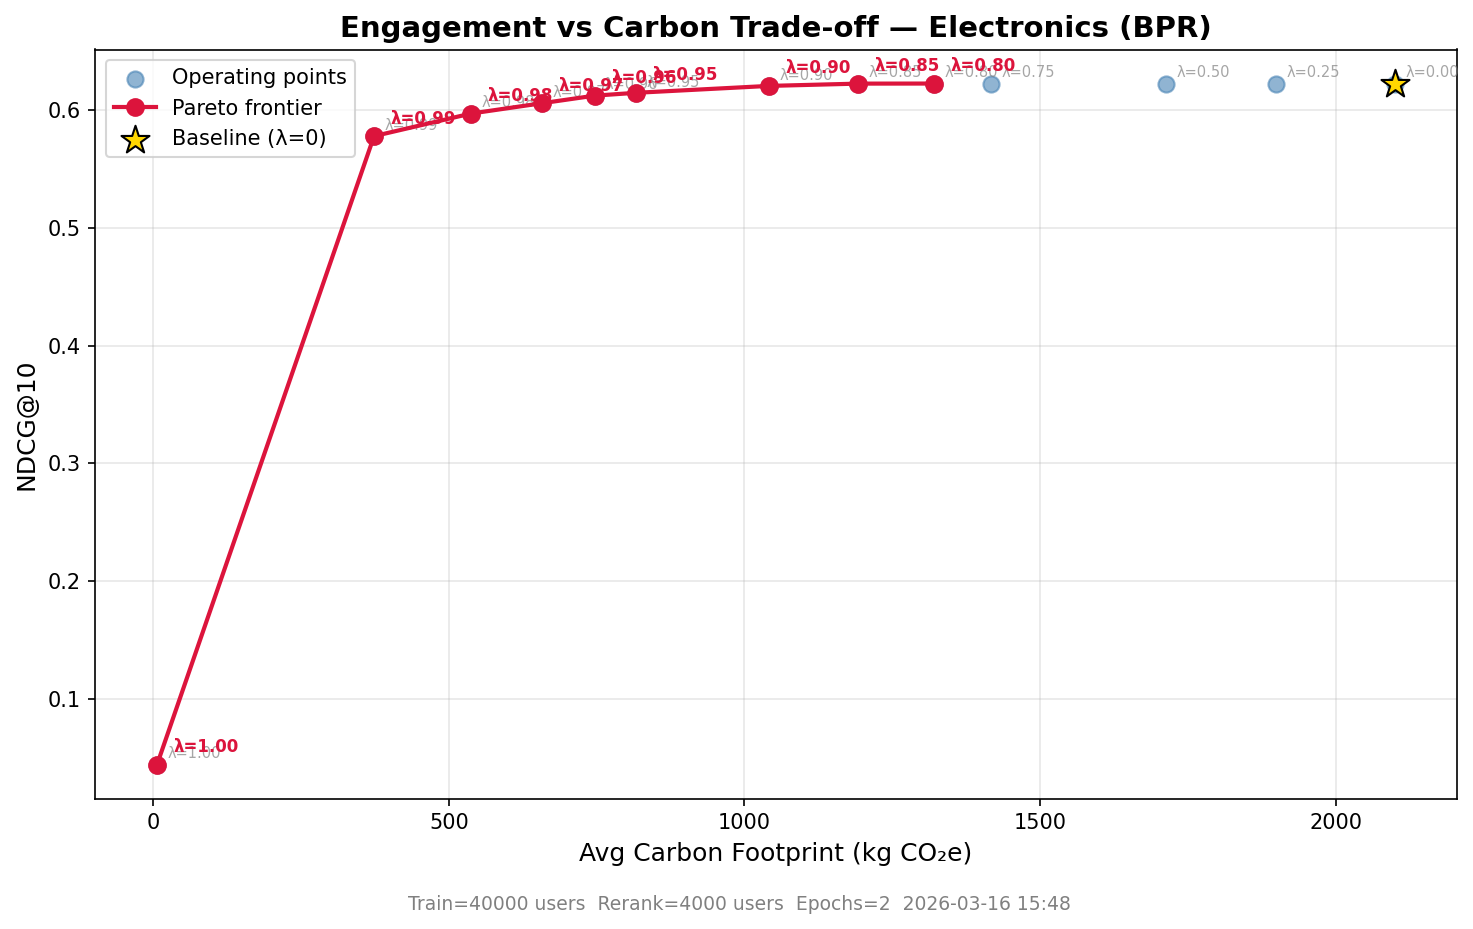
\includegraphics[width=\textwidth]{electronics_BPR_tradeoff}
    \caption{BPR}
  \end{subfigure}
  \hfill
  \begin{subfigure}[t]{0.32\textwidth}
    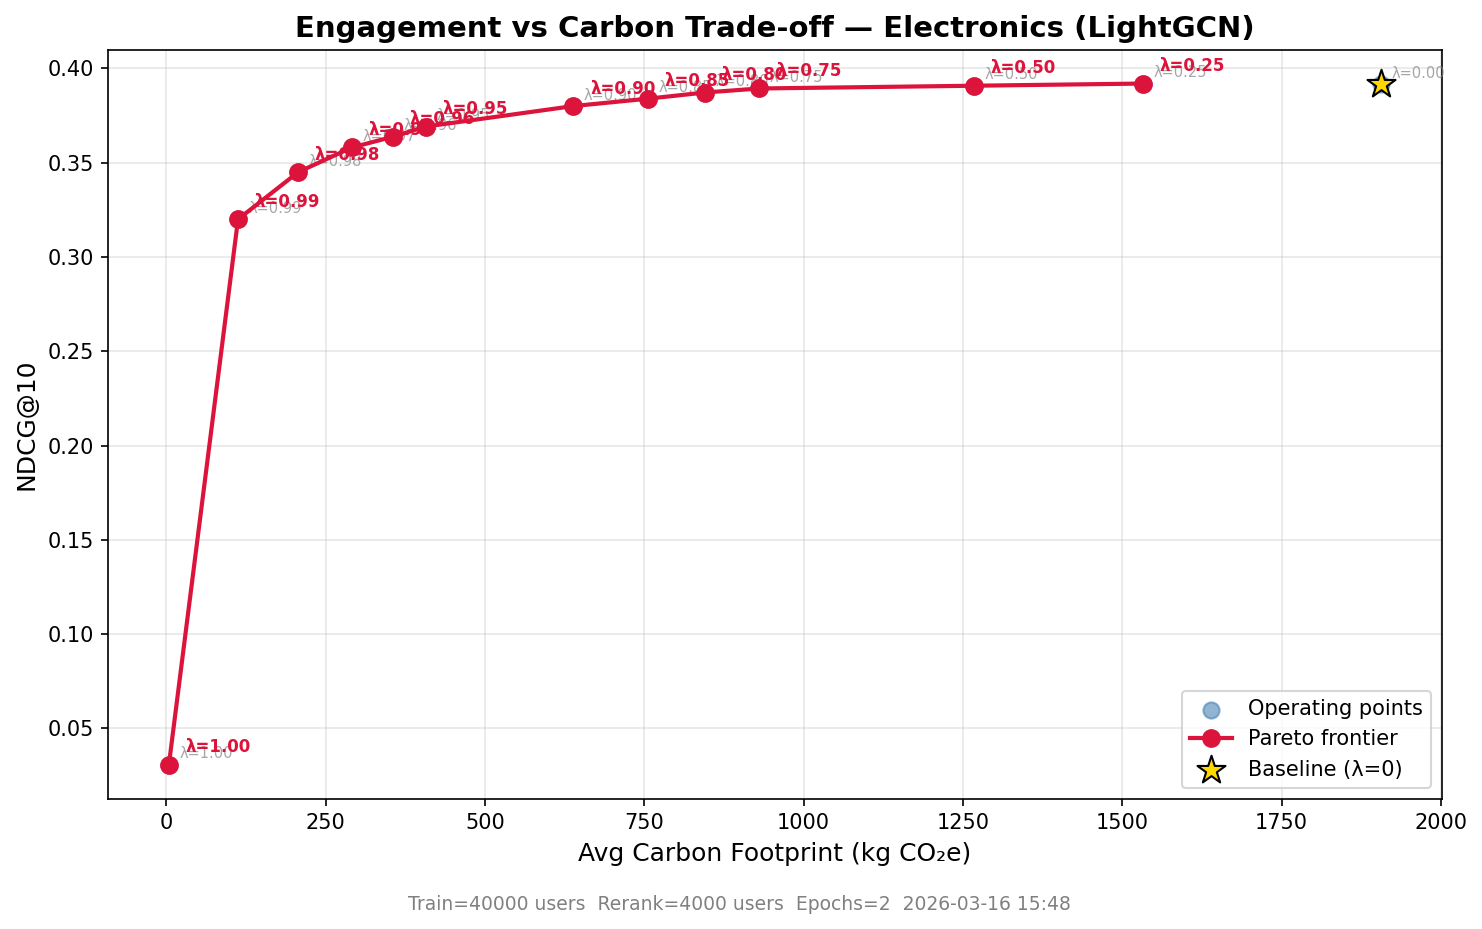
\includegraphics[width=\textwidth]{electronics_LightGCN_tradeoff}
    \caption{LightGCN}
  \end{subfigure}
  \hfill
  \begin{subfigure}[t]{0.32\textwidth}
    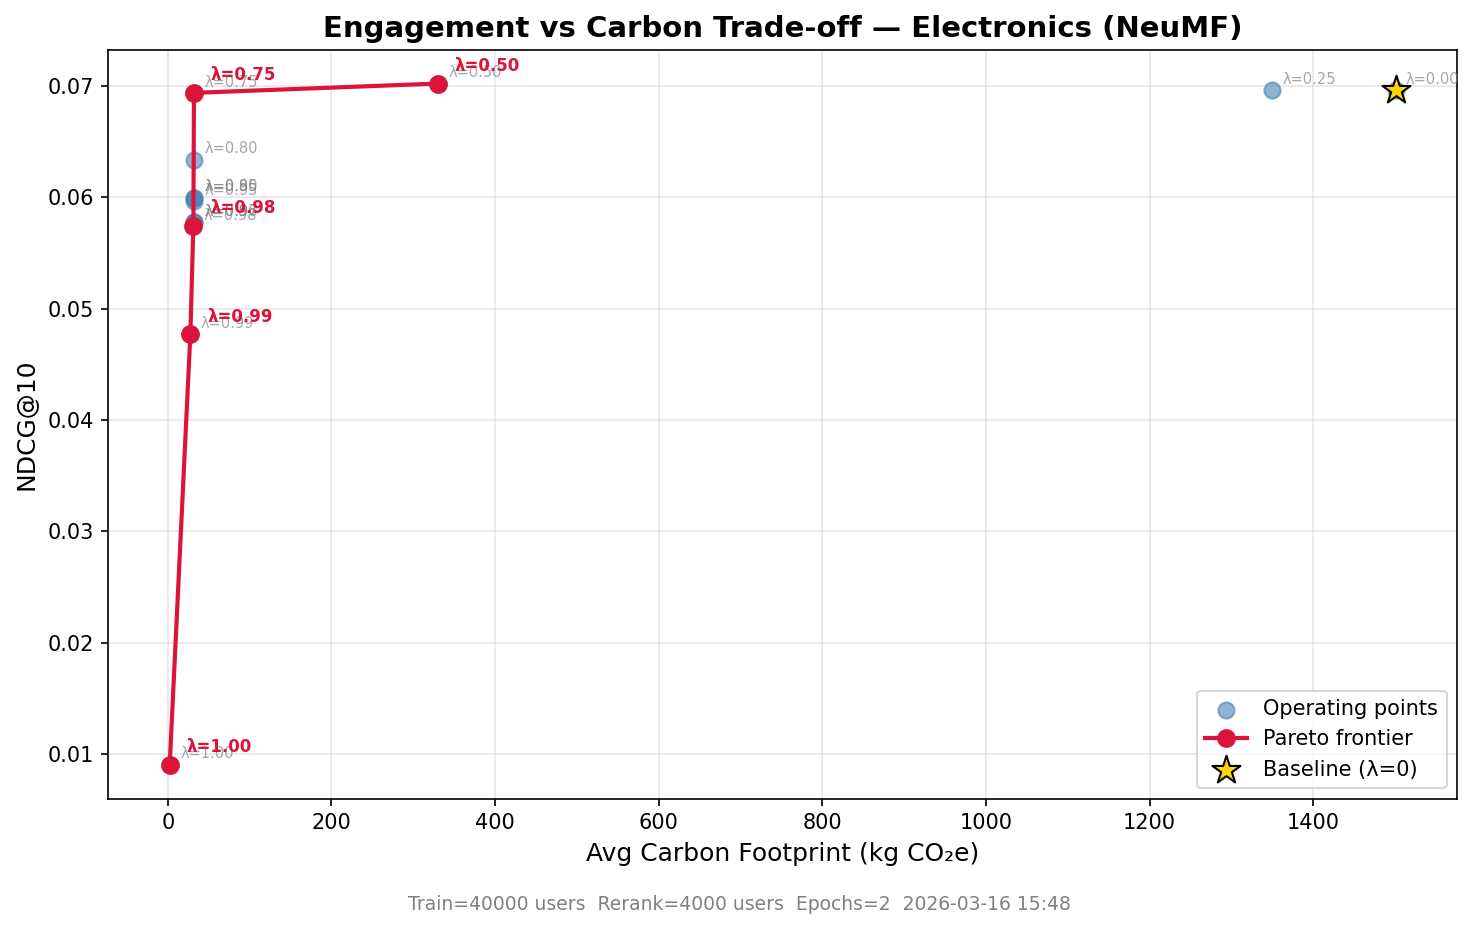
\includegraphics[width=\textwidth]{electronics_NeuMF_tradeoff}
    \caption{NeuMF}
  \end{subfigure}
  \caption{Engagement--carbon Pareto frontiers for Electronics. The star
    marks the engagement-only baseline ($\lambda=0$).}
  \label{fig:tradeoff}
\end{figure}

\begin{figure}[H]
  \centering
  \begin{subfigure}[t]{0.32\textwidth}
    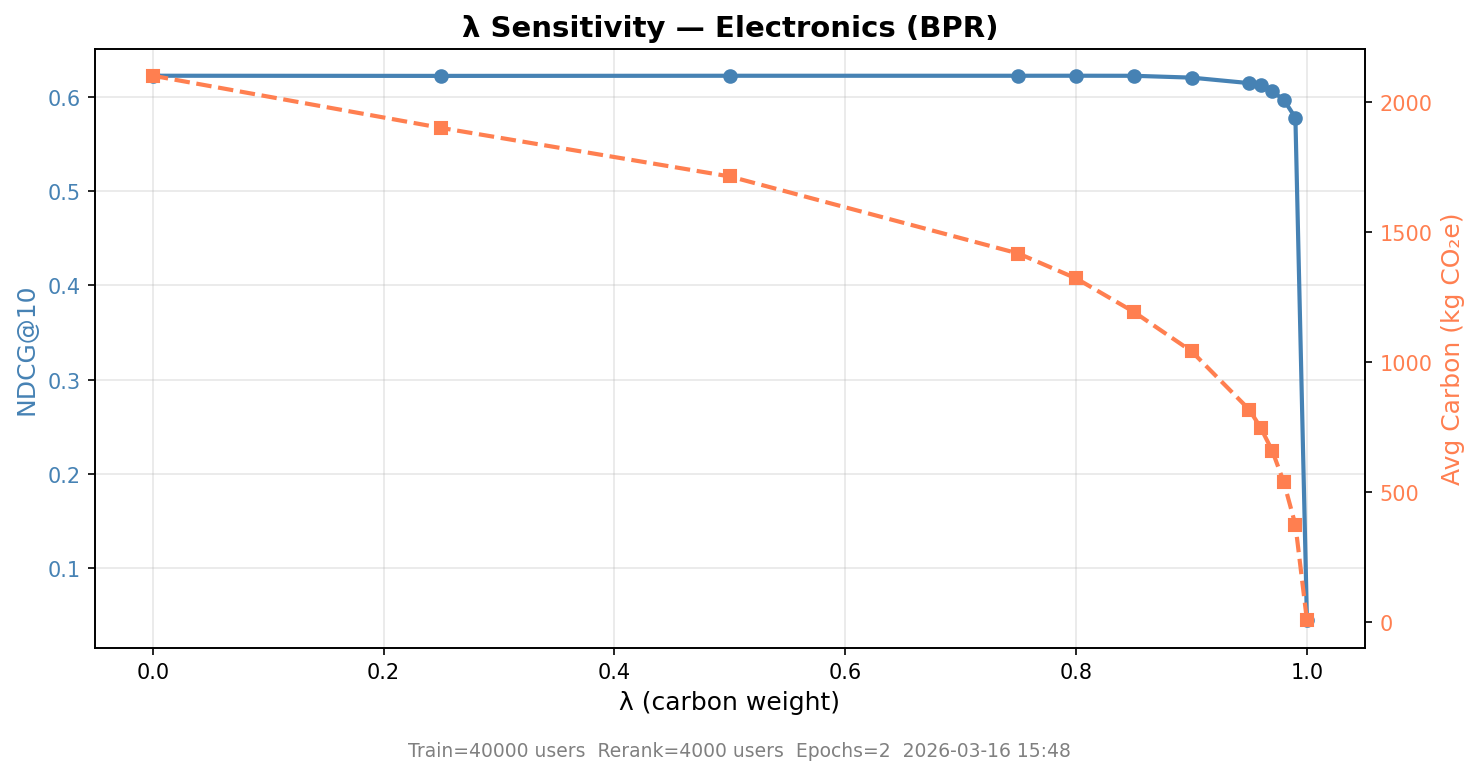
\includegraphics[width=\textwidth]{electronics_BPR_lambda_sensitivity}
    \caption{BPR}
  \end{subfigure}
  \hfill
  \begin{subfigure}[t]{0.32\textwidth}
    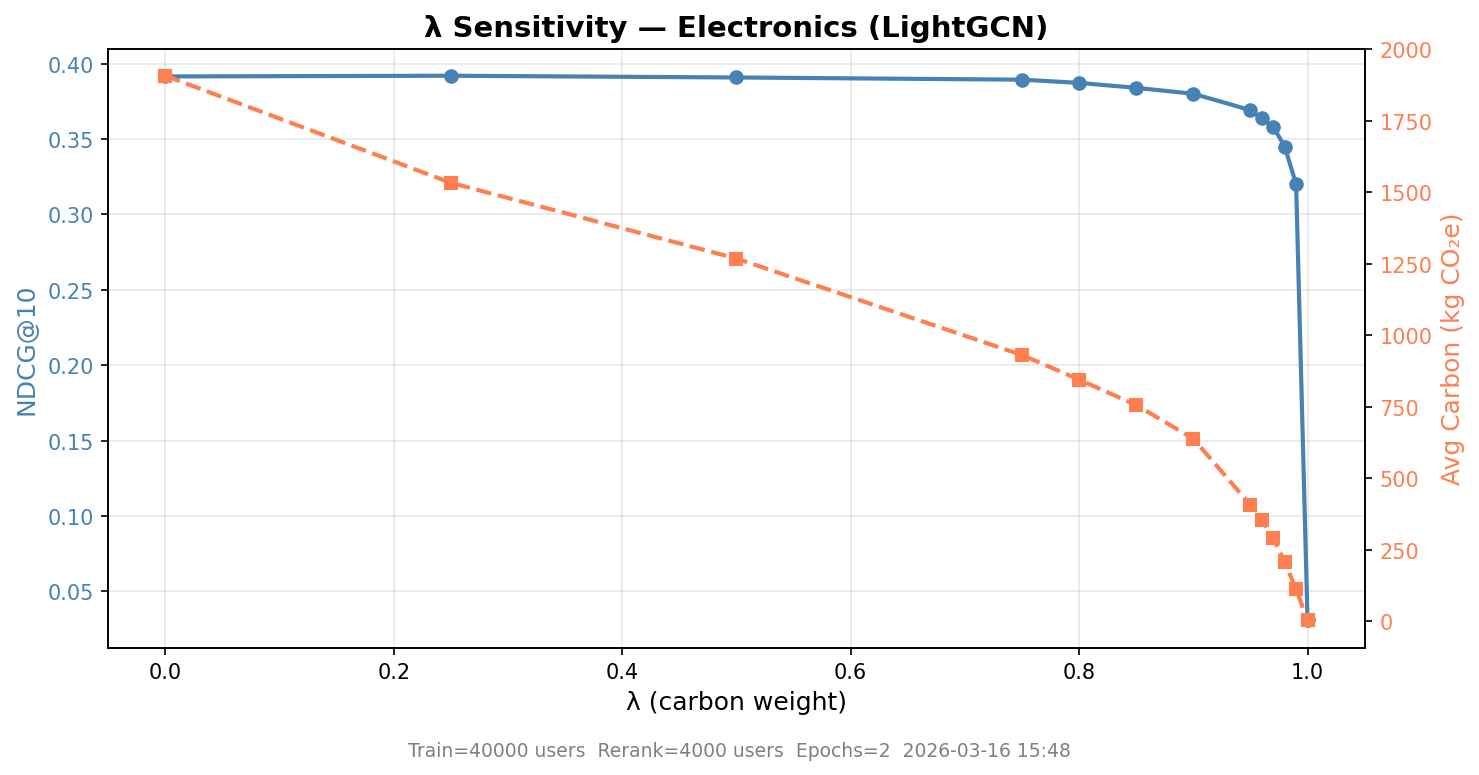
\includegraphics[width=\textwidth]{electronics_LightGCN_lambda_sensitivity}
    \caption{LightGCN}
  \end{subfigure}
  \hfill
  \begin{subfigure}[t]{0.32\textwidth}
    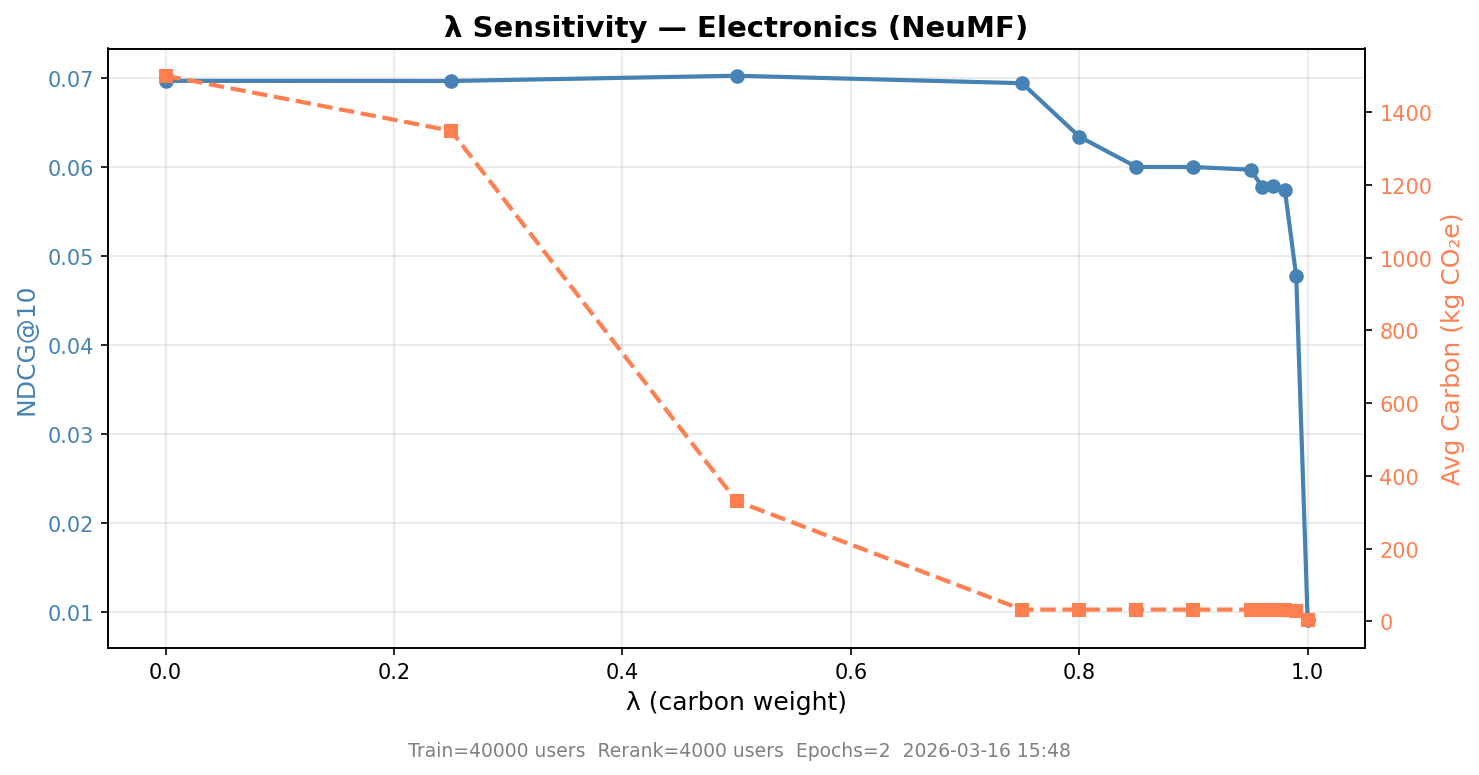
\includegraphics[width=\textwidth]{electronics_NeuMF_lambda_sensitivity}
    \caption{NeuMF}
  \end{subfigure}
  \caption{NDCG@10 (solid, left axis) and AvgPCF@10 (dashed, right axis)
    as a function of $\lambda$. Engagement remains stable across a wide
    range before collapsing near $\lambda = 1$.}
  \label{fig:sensitivity}
\end{figure}

All three models exhibit a consistent \emph{plateau-then-cliff} pattern:
NDCG@10 remains nearly constant for $\lambda \lesssim 0.85{-}0.90$,
then drops sharply near $\lambda = 1$. This structure implies that
substantial carbon reductions are achievable at minimal engagement cost,
a finding consistent with prior sustainability-aware recommendation
work~\cite{spillo2023greenerrec, spillo2023sustainabilityaware}.

\paragraph{BPR.}
BPR achieves the strongest engagement (NDCG@10 = 0.622 at $\lambda=0$)
and maintains it through $\lambda = 0.90$ while reducing average carbon
footprint by over 35\%. The engagement cliff occurs only at
$\lambda \geq 0.95$, making BPR a robust backbone for sustainability-aware
re-ranking in the Electronics category.

\paragraph{LightGCN.}
LightGCN achieves a baseline NDCG@10 of 0.393 and shows a similarly
robust plateau across $\lambda \in [0, 0.85]$, with carbon decreasing
steadily from approximately 1{,}900 to 700\,kg CO$_2$e before the
engagement cliff.

\paragraph{NeuMF.}
NeuMF performs substantially worse in Electronics, with a baseline
NDCG@10 of only 0.070. More notably, its Pareto frontier is qualitatively
different from BPR and LightGCN: engagement degrades much earlier,
beginning at $\lambda \approx 0.75$, producing a sharper curve rather
than the extended plateau seen in the other models.

This warrants further investigation in the final version. We will inspect
raw relevance score distributions for each model to test the score
compression hypothesis directly, and extend NeuMF training to more epochs
to determine how much of the degradation is attributable to underfitting
rather than architectural factors. This directly addresses RQ3 and
motivates careful model selection when deploying carbon-aware re-ranking
in practice~\cite{chaney2018confounding}.

%-----------------------------------------------------------------------
\section{Next Steps}
%-----------------------------------------------------------------------

\begin{itemize}
  \item \textbf{Remaining categories.} Run the full pipeline for Home
    and Kitchen and Sports and Outdoors and report Pareto frontiers and
    $\lambda$ sensitivity curves for all models, enabling the cross-category
    analysis described in RQ2 and RQ3.
  \item \textbf{Carbon unit calibration.} Verify and correctly label
    the units of all AvgPCF@10 values and calibrate the absolute scale
    against real-world LCA benchmarks from the Carbon
    Catalogue.
  \item \textbf{Zero-shot and few-shot variance.} Re-run PCF estimation
    over multiple seeds or the full Carbon Catalogue to report confidence
    intervals and assess stability of the zero-shot vs.\ few-shot gap.
  \item \textbf{NeuMF investigation.} Inspect raw relevance score
    distributions across models to test the score compression hypothesis,
    and retrain NeuMF with additional epochs to disentangle underfitting
    from architectural sensitivity to carbon re-weighting.
  \item \textbf{PCF estimation scale.} Extend the held-out evaluation
    beyond 100 examples to the full Carbon Catalogue or repeated
    fixed-seed subsamples with confidence intervals.
  \item \textbf{Recall@10 reporting.} Add Recall@10 across all models
    and categories in the final version to complement NDCG@10.
  \item \textbf{Synthesis and conclusion.} Compare results across all
    three categories and models, quantify the best Pareto operating
    points, and contextualise findings within the broader literature on
    sustainable recommendation and digital
    nudging.
  \item \textbf{Appendix.} Include hyperparameter configurations for both training and prediction, along with the prompt templates used in the pipeline.
\end{itemize}

\bibliographystyle{plain}
\bibliography{references}

\end{document}
